\chapter{Evaluation}
\label{ch:evaluation}

This chapter describes the experimental evaluation of the MRC system.
First, the simulation environments and test infrastructure are presented
(\autoref{sec:simulation_environment}).
The evaluation methodology, metrics, and automated test protocol are
then defined (\autoref{sec:evaluation_methodology}).
Subsequently, the experimental results are analyzed with respect to
five main dimensions: the comparison of registration backends
(\autoref{sec:backend_comparison}), the impact of pose graph optimization
and topology (\autoref{sec:pose_graph_impact}), the effect of ICP
refinement (\autoref{sec:icp_impact}), a realistic two-robot proximity
scenario (\autoref{sec:proximity_test}), and the scalability of the
system with increasing robot counts
(\autoref{sec:scalability}).
Finally, the key findings are summarized in
\autoref{sec:evaluation_summary}.

%% ---------------------------------------------------------------------------
\section{Simulation Environment}
\label{sec:simulation_environment}

The evaluation was conducted in a physics-based simulation using Gazebo
(Harmonic) with the ROS\,2 Jazzy middleware.
A dedicated ROS\,2 package (\texttt{mrc\_test}) was developed to
provide reproducible, automated benchmarking across a wide range of
configurations and fleet sizes.
Two complementary simulation environments were used: a detailed
indoor room for functional validation and a larger, reduced-physics
environment for scalability testing.

\subsection{Functional Test World}
\label{sec:test_world}

The primary test environment consists of an $8 \times 8$\,m indoor
room with \SI{2.5}{\metre} walls (\autoref{fig:test_world}).
To provide geometric features for LiDAR-based registration, the
room is furnished with several static objects of varying shapes
and sizes: a table ($1.2 \times 0.8$\,m), a chair, a bookshelf
($1.5 \times 0.4 \times 1.8$\,m), a cylindrical trash can
($r = 0.2$\,m), a crate ($0.6^3$\,m), a sphere ($r = 0.15$\,m),
a plant pot, and a square pillar ($0.3 \times 0.3 \times 2.5$\,m).
These objects are distributed asymmetrically to avoid ambiguities
in the registration process.

% TODO: insert screenshot of simulation world
% \begin{figure}[htbp]
%   \centering
%   \includegraphics[width=0.8\textwidth]{figures/mrc_test_world.png}
%   \caption{Gazebo simulation environment: $8 \times 8$\,m room with
%            furniture and obstacles used for functional evaluation.}
%   \label{fig:test_world}
% \end{figure}

Three heterogeneous robots are deployed in an equilateral triangle
formation with a side length of \SI{1.5}{\metre}:
\begin{enumerate}
    \item \textbf{EC Swift~1} (master/reference robot):
          Positioned at $(-0.75, -0.433, 0.15)$\,m with yaw $= 0\degree$.
          Equipped with a single front-facing Livox Mid-360 LiDAR.
    \item \textbf{EC Swift~2}:
          Positioned at $(0.75, -0.433, 0.15)$\,m with yaw $= 120\degree$.
          Equipped with front and back Livox Mid-360 LiDARs, merged
          into a single point cloud.
    \item \textbf{Athena}:
          Positioned at $(0.0, 0.866, 0.15)$\,m with yaw $= -90\degree$.
          Equipped with front and back Livox Mid-360 LiDARs, merged
          into a single point cloud.
\end{enumerate}

\subsection{Scalability Test World}
\label{sec:scale_world}

A second simulation world was designed specifically for evaluating
MRC performance as the fleet size increases.
The scalability world is a $20 \times 20$\,m room with walls and
distributed furniture, using a reduced-physics configuration: only
the ODE physics engine (for stable placement), the sensor rendering
system, and the RGL LiDAR manager are loaded.
IMU and contact simulation are disabled to reduce the computational
overhead per robot and enable simulations with up to 20 simultaneous
robots.

All robots in the scalability tests are homogeneous EC~Swift platforms,
each equipped with a single front-facing Livox Mid-360 LiDAR.
Robot~0 always serves as the master.

\subsection{Predefined Position Configurations}
\label{sec:position_configs}

To ensure systematic and reproducible spatial evaluation, a
comprehensive YAML configuration file defines robot positions
for fleet sizes of $N \in \{2, 3, 5, 7, 10, 12, 15, 17, 20\}$
robots.
For each fleet size, five distinct position setups are provided,
yielding a total of 45 predefined spatial arrangements.
Each position entry specifies $(x, y, z, \psi)$ in meters and
radians.

The five setups per fleet size follow a systematic pattern
designed to exercise different aspects of registration performance:

\begin{description}
    \item[Setup~1: Tight regular polygon.]
        Robots are arranged as a regular $N$-gon with a small
        radius (e.g., \SI{2}{\metre} for 3~robots,
        \SI{5}{\metre} for 20~robots), maximizing inter-robot
        LiDAR overlap.
    \item[Setup~2: Wide regular polygon.]
        The same $N$-gon with a larger radius (e.g., \SI{4}{\metre}
        for 3~robots, \SI{8}{\metre} for 20~robots), testing
        performance under reduced overlap conditions.
    \item[Setup~3: Line/grid formation.]
        Robots are placed in a structured grid or parallel-line
        arrangement (e.g., two rows of five for 10~robots,
        a $5 \times 4$ grid for 20~robots).
    \item[Setup~4: Structured composite.]
        More complex regular patterns such as concentric polygons
        (e.g., inner hexagon + outer hexagon at $30\degree$ offset for
        12~robots), or a center robot with surrounding rings.
    \item[Setup~5: Scattered asymmetric.]
        Robots are placed at irregular, non-symmetric positions
        with varying orientations to test robustness under
        realistic conditions.
\end{description}

Each robot's heading ($\psi$) is varied across setups to create
diverse fields of view.
All positions remain within \SI{8.5}{\metre} of the origin to
fit within the $20 \times 20$\,m room.

\subsection{LiDAR Simulation}

The Livox Mid-360 LiDAR is simulated using the RGL (Robotec GPU
Lidar) Gazebo plugin, which reproduces the non-repetitive scanning
pattern of solid-state LiDARs.
This is a relevant design choice, as the non-repetitive scan pattern
requires temporal accumulation for sufficient spatial coverage, which
is handled by the slave nodes' time-window accumulation mode with
$\Delta t_\mathrm{acc} = \SI{2.0}{\second}$.

%% ---------------------------------------------------------------------------
\section{Evaluation Methodology}
\label{sec:evaluation_methodology}

\subsection{Evaluator Node}
\label{sec:evaluator_node}

An automated evaluator node (\texttt{mrc\_evaluator}, approximately
1\,600 lines of C++) was implemented to enable reproducible
benchmarking.
The evaluator operates within the same TF tree as the master node and
compares the calibrated transforms against the ground truth after each
calibration run.
Key features of the evaluator include:

\begin{itemize}
    \item \textbf{Dynamic robot discovery:}
          In addition to statically configured robot names, the evaluator
          subscribes to the same \texttt{/robot\_announcement} topic as
          the master node.
          When a new \texttt{RobotAnnouncement} message is received,
          the evaluator automatically registers the robot, loads its
          ground truth from launch-file parameters, and creates per-robot
          error publishers.
          This enables seamless evaluation of variable fleet sizes without
          manual configuration changes.

    \item \textbf{Ground truth from spawn positions:}
          Ground truth poses are derived from the known Gazebo spawn
          positions, transformed into the master robot's
          \texttt{base\_link} frame.
          For the scalability tests, the launch file computes ground
          truth positions as:
          \begin{equation}
              \mathbf{p}_\mathrm{gt}^{(i)} = \mathbf{R}(-\psi_0)
              \cdot (\mathbf{p}_i - \mathbf{p}_0), \qquad
              \psi_\mathrm{gt}^{(i)} = \psi_i - \psi_0
          \end{equation}
          where $(\mathbf{p}_0, \psi_0)$ is the master's world pose
          and $(\mathbf{p}_i, \psi_i)$ is the $i$-th slave's world pose.

    \item \textbf{Voxel-based overlap computation:}
          The evaluator can compute the point cloud overlap ratio between
          each slave robot and the master.
          The overlap is computed by voxelizing both point clouds
          (retrieved from the slave nodes' \texttt{get\_registration\_data}
          service) at a configurable resolution
          ($v = \SI{0.25}{\metre}$ by default) using a hash-map of
          integer voxel keys.
          The overlap ratio for slave $i$ is:
          \begin{equation}
              o^{(i)} = \frac{|V_\mathrm{master} \cap V_i|}{|V_i|}
          \end{equation}
          where $V_\mathrm{master}$ and $V_i$ are the occupied voxel
          sets of the master and slave point clouds, respectively,
          after transforming the slave cloud by the ground truth pose.
          This metric quantifies how much of the slave's observed
          environment is also visible to the master---a key indicator
          of registration feasibility.

    \item \textbf{Runtime parameter reconfiguration:}
          The evaluator modifies MRC master parameters (algorithm,
          pose graph mode, topology, ICP refinement) at runtime via
          the ROS\,2 parameter service, enabling all 12 configurations
          to be tested within a single simulation session without
          restarting nodes.
\end{itemize}

The evaluator exposes five ROS\,2 service interfaces for different
evaluation modes:
\begin{description}
    \item[\texttt{trigger\_evaluation}:]
        Triggers a single calibration run followed by evaluation.
    \item[\texttt{trigger\_pose\_graph\_comparison}:]
        Compares three pose graph modes (none, star, mesh) using
        multiple trials with the current algorithm.
    \item[\texttt{trigger\_full\_comparison}:]
        Tests all 6 backend-and-topology combinations
        ($2$ algorithms $\times$ $3$ pose graph modes).
    \item[\texttt{trigger\_icp\_comparison}:]
        Compares coarse-only registration against coarse + ICP
        refinement for the current configuration.
    \item[\texttt{trigger\_comprehensive\_comparison}:]
        Full factorial evaluation of all $2 \times 3 \times 2 = 12$
        parameter combinations (2~algorithms $\times$ 3~pose graph
        modes $\times$ 2~ICP settings), each repeated over $k$ trials.
\end{description}

\subsection{Metrics}
\label{sec:metrics}

For each calibrated robot $i$, the following error metrics are computed
against the ground truth:

\paragraph{Translation error.}
The Euclidean distance between the estimated and ground truth positions:
\begin{equation}
    e_t^{(i)} = \lVert \mathbf{p}_\mathrm{est}^{(i)}
                      - \mathbf{p}_\mathrm{gt}^{(i)} \rVert_2
\end{equation}

\paragraph{Rotation error.}
The absolute yaw angle difference, normalized to $[-\pi, \pi]$:
\begin{equation}
    e_r^{(i)} = \left| \psi_\mathrm{est}^{(i)}
                     - \psi_\mathrm{gt}^{(i)} \right|
\end{equation}

These per-robot errors are aggregated into the following summary
statistics over $n$ valid robots:
\begin{itemize}
    \item \textbf{Mean translation error:}
          $\bar{e}_t = \frac{1}{n} \sum_{i=1}^{n} e_t^{(i)}$
    \item \textbf{RMS translation error:}
          $e_t^\mathrm{RMS} = \sqrt{\frac{1}{n} \sum_{i=1}^{n}
          (e_t^{(i)})^2}$
    \item \textbf{Maximum translation error:}
          $e_t^\mathrm{max} = \max_i \, e_t^{(i)}$
    \item \textbf{Mean rotation error:}
          $\bar{e}_r = \frac{1}{n} \sum_{i=1}^{n} e_r^{(i)}$
    \item \textbf{Mean overlap ratio:}
          $\bar{o} = \frac{1}{n} \sum_{i=1}^{n} o^{(i)}$
\end{itemize}

\subsection{Test Protocol and Automation}
\label{sec:test_protocol}

Each configuration was evaluated using $k = 3$ independent calibration
trials.
The reported metrics are averaged across trials to reduce the influence
of stochastic effects (e.g., variations in accumulated point clouds
due to the non-repetitive LiDAR pattern).
Between each trial, a delay of \SI{5.5}{\second} was introduced to
ensure TF propagation.

The configurations tested span the full combinatorial space of the
MRC system parameters:
\begin{itemize}
    \item \textbf{Registration backend:} KISS-Matcher, FRICP
    \item \textbf{Pose graph optimization:} disabled, star topology,
          mesh topology
    \item \textbf{ICP refinement:} disabled, enabled
\end{itemize}
This yields $2 \times 3 \times 2 = 12$ configurations, each
evaluated with $k$ trials, for a total of $12k$ calibration runs
per test setup.

\paragraph{Automated test suite.}
A Bash orchestration script (\texttt{run\_all\_mrc\_tests.bash})
automates the complete evaluation across multiple robot counts and
position setups.
The script performs the following sequence:
\begin{enumerate}
    \item For each robot count $N \in \{3, 5, 10\}$ and each position
          setup $s \in \{1, 2, 3, 4, 5\}$, launch the corresponding
          simulation environment with $N$ robots at the predefined
          positions.
    \item Wait for all \texttt{robot\_description} topics to appear
          (with a \SI{90}{\second} timeout) to confirm successful
          robot spawning.
    \item Trigger the comprehensive comparison service on the evaluator
          node, which internally runs all 12 parameter combinations
          with $k$ trials each.
    \item Monitor the log output for a completion marker
          (\texttt{BEST CONFIGURATION}), with a per-test timeout
          of \SI{1000}{\second}.
    \item Extract structured results from the log output using
          AWK-based parsers into CSV files:
          \begin{itemize}
              \item \texttt{results.csv}: aggregated per-configuration
                    metrics across all tests
              \item \texttt{details.csv}: per-trial metrics for each
                    configuration
              \item \texttt{registrations.csv}: per-robot, per-trial
                    registration data including pose graph edge quality
                    metrics (RMSE, inliers, sigma)
          \end{itemize}
    \item Clean up all ROS and Gazebo processes between tests
          (including a ROS\,2 daemon restart to clear stale
          discovery state).
\end{enumerate}

The default test matrix comprises $3$ robot counts $\times$
$5$ position setups $= 15$ tests, each evaluating 12~configurations
with $k = 3$~trials, for a total of $15 \times 12 \times 3 = 540$
calibration runs.
All results are written to a timestamped output directory.

\paragraph{Visualization pipeline.}
A Python visualization script (\texttt{visualize\_mrc\_results.py})
automatically generates publication-quality plots from the CSV output:
\begin{itemize}
    \item Bar charts comparing all 12~configurations on translation
          error (average, RMS), rotation error, and computation time.
    \item Grouped bar charts contrasting unoptimized (no~PG) vs.\
          optimized (star, mesh) configurations per algorithm.
    \item Pose graph topology visualizations showing robot positions
          with edges for star and mesh topologies, annotated with
          the best-performing metrics.
    \item Heatmaps of translation RMS across robot counts and
          position setups for each configuration.
    \item Summary bar charts of translation RMS averaged across
          position setups, grouped by robot count.
\end{itemize}

%% ---------------------------------------------------------------------------
\section{Results: Backend Comparison}
\label{sec:backend_comparison}

\autoref{tab:results_overview} presents the full results for all 12
configurations, averaged across all position setups and robot counts
($N \in \{3, 5\}$, 5~setups each, 3~trials per configuration).

\begin{table}[htbp]
    \centering
    \caption{Calibration results for all 12 configurations
             (averaged over $N \in \{3, 5\}$ robots, 5~position setups
             each, and 3~trials per configuration).}
    \label{tab:results_overview}
    \small
    \begin{tabular}{l r r r r r}
        \toprule
        \textbf{Configuration}
            & $\bar{e}_t$ [m]
            & $e_t^\mathrm{RMS}$ [m]
            & $e_t^\mathrm{max}$ [m]
            & $\bar{e}_r$ [deg]
            & $t$ [s] \\
        \midrule
        \multicolumn{6}{l}{\textit{KISS-Matcher}} \\
        \quad no PG             & \textbf{2.58}  & \textbf{3.04}  & 5.55
                                & \textbf{46.8}  & 0.14 \\
        \quad star PG           & 3.45  & 4.05  & 5.88  & 66.8  & 0.21 \\
        \quad mesh PG           & 4.16  & 4.72  & 6.76  & 83.4  & 0.19 \\
        \quad no PG + ICP       & 3.87  & 4.56  & 7.00  & 79.4  & 1.70 \\
        \quad star PG + ICP     & 3.93  & 4.92  & 7.36  & 76.3  & 1.70 \\
        \quad mesh PG + ICP     & 3.92  & 4.71  & 7.75  & 81.6  & 3.62 \\
        \midrule
        \multicolumn{6}{l}{\textit{FRICP}} \\
        \quad no PG             & 5.48  & 5.93  & 7.82  & 131.1 & 2.97 \\
        \quad star PG           & 5.95  & 6.30  & 7.82  & 143.1 & 2.99 \\
        \quad mesh PG           & 6.20  & 6.45  & 7.82  & 146.5 & 6.91 \\
        \quad no PG + ICP       & 6.02  & 6.37  & 7.84  & 150.6 & 5.40 \\
        \quad star PG + ICP     & 5.99  & 6.36  & 7.84  & 153.6 & 5.41 \\
        \quad mesh PG + ICP     & 6.18  & 6.54  & 8.05  & 148.9 & 12.14 \\
        \bottomrule
    \end{tabular}
\end{table}

In a head-to-head comparison across all six pose-graph and ICP
combinations, KISS-Matcher consistently outperformed FRICP
(\autoref{tab:head_to_head}).

\begin{table}[htbp]
    \centering
    \caption{Head-to-head comparison of registration backends
             ($e_t^\mathrm{RMS}$ in meters, averaged over all experiments).}
    \label{tab:head_to_head}
    \begin{tabular}{l r r l}
        \toprule
        \textbf{Configuration}
            & \textbf{KISS-Matcher}
            & \textbf{FRICP}
            & \textbf{Winner} \\
        \midrule
        no PG           & 3.04  & 5.93  & KISS-Matcher \\
        star PG         & 4.05  & 6.30  & KISS-Matcher \\
        mesh PG         & 4.72  & 6.45  & KISS-Matcher \\
        no PG + ICP     & 4.56  & 6.37  & KISS-Matcher \\
        star PG + ICP   & 4.92  & 6.36  & KISS-Matcher \\
        mesh PG + ICP   & 4.71  & 6.54  & KISS-Matcher \\
        \bottomrule
    \end{tabular}
\end{table}

The superior performance of KISS-Matcher can be attributed to two
factors:
(1)~the feature-based approach provides a global registration
capability that does not require an initial pose estimate, whereas
FRICP starts from the identity transform and may converge to local
minima; and
(2)~the robust GNC-TLS solver in KISS-Matcher effectively handles
outlier correspondences, whereas FRICP's Welsch cost function, while
robust, is sensitive to the initial alignment.

The FRICP backend consistently exhibited large rotation errors
($> 100\degree$), indicating frequent convergence to incorrect local
minima.
This is expected behavior for an ICP-variant applied without a
reasonable initial guess in scenarios with limited overlap.

\paragraph{Computation time.}
KISS-Matcher completed registration in approximately
\SIrange{0.1}{0.2}{\second}, while FRICP required
\SIrange{3.0}{7.0}{\second} per calibration run (increasing with
mesh topology due to $\binom{N}{2}$ pairwise registrations).
The $> 20\times$ speedup of KISS-Matcher is due to operating
on a compact set of keypoints and descriptors rather than the full
dense point cloud.

%% ---------------------------------------------------------------------------
\section{Results: Pose Graph Optimization}
\label{sec:pose_graph_impact}

The impact of pose graph optimization was evaluated by comparing
three modes: no pose graph (direct pairwise registration), star
topology, and mesh topology.
\autoref{tab:pg_impact} summarizes the relative changes, averaged
across all experiments ($N \in \{3, 5\}$, 5~setups each).

\begin{table}[htbp]
    \centering
    \caption{Pose graph optimization impact on translation RMS error,
             averaged over all experiments
             (positive values indicate improvement over the baseline).}
    \label{tab:pg_impact}
    \begin{tabular}{l r r r}
        \toprule
        \textbf{Backend}
            & \textbf{Star vs.\ None}
            & \textbf{Mesh vs.\ Star}
            & \textbf{Mesh vs.\ None} \\
        \midrule
        KISS-Matcher       & $-33.4\%$ & $-16.4\%$ & $-55.3\%$ \\
        KISS-Matcher + ICP & $-7.8\%$  & $+4.2\%$  & $-3.3\%$ \\
        FRICP              & $-6.3\%$  & $-2.3\%$  & $-8.7\%$ \\
        FRICP + ICP        & $+0.2\%$  & $-2.9\%$  & $-2.7\%$ \\
        \bottomrule
    \end{tabular}
\end{table}

When averaged across all position setups and fleet sizes,
pose graph optimization generally degraded calibration accuracy
for both backends.
For KISS-Matcher without ICP, star topology increased the
translation RMS by 33.4\% (from \SI{3.04}{\metre} to
\SI{4.05}{\metre}), and mesh topology worsened it further by 55.3\%.
This contrasts with single-setup results where star topology can
improve accuracy, indicating that the benefit of pose graph
optimization is highly setup-dependent.
In setups where some pairwise registrations converge to incorrect
local minima, the pose graph optimizer propagates these errors
through the graph rather than correcting them.

For the FRICP backend, pose graph optimization similarly degraded
the results, though the effect is less pronounced ($\leq 9\%$).
This is because FRICP registrations are already unreliable due to
local-minimum convergence issues, and the additional constraints
from the pose graph cannot compensate for the poor edge quality.
The only configuration where pose graph optimization provided
a small benefit was KISS-Matcher with ICP refinement, where mesh
topology improved by 4.2\% over star---suggesting that in cases
where ICP can refine individual edges, the additional mesh
constraints help average out residual errors.

%% ---------------------------------------------------------------------------
\section{Results: ICP Refinement}
\label{sec:icp_impact}

Contrary to expectations, the optional ICP refinement stage
consistently degraded calibration accuracy in the multi-robot
distributed scenario when averaged across all experiments
(\autoref{tab:icp_impact}).

\begin{table}[htbp]
    \centering
    \caption{ICP refinement impact on translation RMS error,
             averaged over all experiments.
             Negative values indicate degradation.}
    \label{tab:icp_impact}
    \begin{tabular}{l r r l}
        \toprule
        \textbf{Backend + PG}
            & \textbf{Coarse} [m]
            & \textbf{+ ICP} [m]
            & \textbf{Change} \\
        \midrule
        KISS-Matcher, no PG   & 3.04  & 4.56  & $-50.2\%$ \\
        KISS-Matcher, star    & 4.05  & 4.92  & $-21.4\%$ \\
        KISS-Matcher, mesh    & 4.72  & 4.71  & $-0.1\%$  \\
        FRICP, no PG          & 5.93  & 6.37  & $-7.4\%$  \\
        FRICP, star           & 6.30  & 6.36  & $-0.9\%$  \\
        FRICP, mesh           & 6.45  & 6.54  & $-1.5\%$  \\
        \bottomrule
    \end{tabular}
\end{table}

The largest degradation ($-50.2\%$) occurs for KISS-Matcher without
pose graph, where ICP shifts the coarse feature-based alignment
toward locally dense regions.
For FRICP, the effect is smaller ($\leq 7.4\%$) because the coarse
result is already poor.
The only near-neutral case is KISS-Matcher with mesh topology,
where the pose graph provides sufficient constraints that ICP
refinement neither helps nor hinders ($-0.1\%$).

This negative result can be explained by the characteristics of the
multi-robot scenario:
the solid-state LiDAR produces sparse, non-uniformly distributed
point clouds with limited overlap between distant robots.
Standard ICP minimizes point-to-point distances, which can shift
the alignment toward locally dense regions (e.g., nearby walls)
rather than preserving the globally correct feature-based alignment.
The conservative acceptance criterion in the ICP refiner (reject if
RMSE worsens) should prevent degradation; however, the RMSE metric
itself can be misleading when the nearest-neighbor correspondences
are systematically biased by the non-uniform point distribution.

%% ---------------------------------------------------------------------------
\section{Realistic Proximity Scenario}
\label{sec:proximity_test}

While the multi-robot scalability tests evaluate MRC under a wide
range of fleet sizes and spatial configurations, the most common
real-world use case for extrinsic multi-robot calibration involves
exactly two robots placed side by side---for example, to determine
the static transform between two map frames for cooperative
navigation.
A dedicated proximity test was designed to evaluate MRC under
these realistic operating conditions.

\subsection{Test Setup}

The proximity test uses the \texttt{mrc\_icp\_pg\_test\_2} launch
file, which spawns two homogeneous EC~Swift robots, each equipped
with both front and back Livox Mid-360 LiDARs (providing
$360\degree$ coverage).
The simulation uses a headless Gazebo instance (\texttt{-s} flag)
with the lightweight lidar-only world
(\texttt{pose\_graph\_scale\_room\_lidar\_only.sdf}), which
removes the ogre2 render engine entirely since RGL performs its
own GPU raytracing independently.
Physics are reduced to \SI{100}{\hertz} (from \SI{250}{\hertz})
as the robots are static.
This optimized setup significantly reduces computational overhead,
enabling faster test execution.

The robots are placed in proximity configurations that simulate
real-world placement uncertainty.
Five predefined setups are provided, all featuring two robots
facing approximately the same direction with lateral separations
of \SIrange{0.8}{2.0}{\metre}:

\begin{table}[htbp]
    \centering
    \caption{Two-robot proximity test position setups.
             Robot~0 (master) is at the origin in all setups.}
    \label{tab:proximity_setups}
    \small
    \begin{tabular}{c l c c}
        \toprule
        \textbf{Setup}
            & \textbf{Description}
            & \textbf{Distance} [m]
            & $\Delta\psi$ [deg] \\
        \midrule
        1 & Parallel, no noise     & 1.5  & $0.0$ \\
        2 & Slight offset + yaw    & 1.0  & $2.9$ \\
        3 & Behind + small yaw     & 2.0  & $-4.6$ \\
        4 & Both with yaw noise    & 1.2  & $-4.6$ \\
        5 & Very close, more noise & 0.8  & $5.7$ \\
        \bottomrule
    \end{tabular}
\end{table}

Unlike the scalability tests where each robot uses only a single
front LiDAR, the proximity test equips each robot with both front
and back LiDARs, merging them into a single $360\degree$ point
cloud per robot.
This mirrors the real deployment configuration and maximizes
point cloud overlap between the two platforms.

\subsection{Evaluation Protocol}

The comprehensive comparison is triggered automatically after
all nodes are initialized (with a \SI{20}{\second} stabilization
delay after the evaluator launches).
All 12 parameter combinations are tested:
\begin{equation*}
    \underbrace{2}_\text{algorithms}
    \times
    \underbrace{3}_\text{PG modes}
    \times
    \underbrace{2}_\text{ICP options}
    = 12 \text{ configurations}
\end{equation*}
each with $k = 3$ trials, for a total of 36 calibration runs per
position setup.

In the two-robot case ($N = 2$), the pose graph reduces to:
\begin{itemize}
    \item \textbf{No PG:} Direct pairwise registration
          (master $\to$ slave).
    \item \textbf{Star:} Identical to no PG for $N = 2$, since
          the star topology has only one edge
          (master $\leftrightarrow$ slave).
    \item \textbf{Mesh:} Also identical for $N = 2$, since
          $\binom{2}{2} = 1$ edge.
\end{itemize}
Thus, the three pose graph modes are expected to produce equivalent
results in this scenario, effectively isolating the impact of the
registration algorithm and ICP refinement.

\subsection{Results}

\autoref{tab:proximity_results} presents the full results for all
12 configurations, averaged across the five position setups and
three trials per configuration.
The point cloud overlap across setups ranged from 60.8\% (Setup~3,
\SI{2.0}{\metre} separation) to 70.5\% (Setup~5, \SI{0.8}{\metre}
separation).

\begin{table}[htbp]
    \centering
    \caption{Proximity test results (2 robots, averaged over 5 setups
             and 3 trials per configuration).}
    \label{tab:proximity_results}
    \small
    \begin{tabular}{l r r r}
        \toprule
        \textbf{Configuration}
            & $\bar{e}_t$ [m]
            & $\bar{e}_r$ [deg]
            & $t$ [s] \\
        \midrule
        \multicolumn{4}{l}{\textit{KISS-Matcher}} \\
        \quad no PG             & 0.1262  & 1.61  & 0.10 \\
        \quad star PG           & 0.1583  & 2.00  & 0.08 \\
        \quad mesh PG           & 0.1519  & 2.37  & 0.10 \\
        \quad no PG + ICP       & 0.1554  & 2.44  & 0.64 \\
        \quad star PG + ICP     & 0.0667  & 0.91  & 0.62 \\
        \quad mesh PG + ICP     & 0.0330  & 0.41  & 0.64 \\
        \midrule
        \multicolumn{4}{l}{\textit{FRICP}} \\
        \quad no PG             & 0.0139  & 0.15  & 0.74 \\
        \quad star PG           & 0.0074  & 0.06  & 0.82 \\
        \quad mesh PG           & \textbf{0.0062}  & \textbf{0.03}  & 0.74 \\
        \quad no PG + ICP       & 0.0192  & 0.11  & 1.30 \\
        \quad star PG + ICP     & 0.0248  & 0.14  & 1.24 \\
        \quad mesh PG + ICP     & 0.0255  & 0.15  & 1.26 \\
        \bottomrule
    \end{tabular}
\end{table}

\paragraph{FRICP dominates in the proximity scenario.}
In stark contrast to the multi-robot results
(\autoref{sec:backend_comparison}), FRICP consistently and
significantly outperformed KISS-Matcher in all 12 configurations.
The best configuration overall was \textbf{FRICP with mesh PG},
achieving a mean translation error of only \SI{6.2}{\milli\metre}
and a mean rotation error of $0.03\degree$.
Even the worst FRICP configuration
(mesh PG + ICP, $\bar{e}_t = \SI{25.5}{\milli\metre}$) outperformed
the best KISS-Matcher configuration without ICP
($\bar{e}_t = \SI{126}{\milli\metre}$).

This result reversal is explained by the favorable conditions
of the proximity scenario:
\begin{enumerate}
    \item \textbf{High point cloud overlap} (59--69\%) from
          $360\degree$ LiDAR coverage and short inter-robot distances
          (\SIrange{0.8}{2.0}{\metre}).
    \item \textbf{Small relative yaw} ($< 6\degree$), so FRICP's
          initialization from the identity transform is already close
          to the correct solution, avoiding local minima.
    \item \textbf{Dense geometric constraints} --- both robots observe
          largely the same environment, providing rich correspondences
          for the iterative Welsch cost minimization.
\end{enumerate}
Under these conditions, FRICP converges reliably to the global
optimum, and its dense point-to-point optimization achieves
sub-centimeter accuracy.
KISS-Matcher, by contrast, operates on quantized feature
descriptors (FasterPFH) and exhibits an accuracy floor of
approximately \SI{10}{\centi\metre} inherent to the feature-based
approach.

\paragraph{ICP refinement helps KISS-Matcher but hinders FRICP.}
This result is the inverse of the multi-robot test
(\autoref{sec:icp_impact}).
For KISS-Matcher, ICP refinement reduced the mean translation error
by 58--78\% when combined with pose graph optimization, with the
largest improvement for mesh PG (from \SI{152}{\milli\metre} to
\SI{33}{\milli\metre}).
The high overlap and favorable geometry ensure that the ICP
refinement stage has sufficient correspondences to improve upon
the coarse feature-based estimate.

For FRICP, however, ICP refinement consistently degraded accuracy.
With mesh PG, the translation error increased from
\SI{6.2}{\milli\metre} to \SI{25.5}{\milli\metre}---a $4.1\times$
degradation.
This occurs because FRICP's Welsch cost optimization already
converges to a near-perfect solution; the subsequent ICP pass
uses a standard point-to-point objective that introduces
systematic bias from the non-uniform LiDAR point distribution.

\paragraph{Consistency across setups.}
\autoref{tab:proximity_per_setup} shows the best configuration's
translation error for each position setup, demonstrating
consistent sub-centimeter accuracy across all spatial arrangements.

\begin{table}[htbp]
    \centering
    \caption{Best configuration (FRICP, mesh PG) per position setup
             (translation error averaged over 3 trials).}
    \label{tab:proximity_per_setup}
    \small
    \begin{tabular}{c c c c c}
        \toprule
        \textbf{Setup}
            & \textbf{Distance} [m]
            & $\bar{e}_t$ [mm]
            & $\bar{e}_r$ [deg]
            & \textbf{Overlap} [\%] \\
        \midrule
        1 & 1.5  &  2.6  & 0.01  & 66.0 \\
        2 & 1.0  &  9.5  & 0.05  & 69.7 \\
        3 & 2.0  &  5.9  & 0.03  & 60.8 \\
        4 & 1.2  &  4.4  & 0.02  & 64.7 \\
        5 & 0.8  &  8.4  & 0.06  & 70.5 \\
        \midrule
        \multicolumn{2}{c}{\textbf{Average}} & \textbf{6.2} & \textbf{0.03} & \textbf{66.3} \\
        \bottomrule
    \end{tabular}
\end{table}

The lowest error (\SI{2.6}{\milli\metre}) was achieved in Setup~1,
the parallel arrangement at \SI{1.5}{\metre} separation.
Setup~2 exhibited the highest error (\SI{9.5}{\milli\metre}),
likely due to the combined forward offset and yaw perturbation
creating a slightly more challenging registration geometry.
Notably, all five setups achieved sub-centimeter accuracy,
confirming that MRC reliably determines the relative pose
between two closely placed robots.

\paragraph{Comparison with multi-robot results.}
The proximity test reveals that MRC's optimal configuration
depends fundamentally on the deployment scenario:
\begin{itemize}
    \item \textbf{Multi-robot distributed ($N \geq 3$):}
          KISS-Matcher without pose graph is recommended
          ($\bar{e}_t \approx \SI{2.58}{\metre}$), as FRICP
          fails due to local minima in the absence of a good
          initial estimate.
    \item \textbf{Two-robot proximity ($N = 2$):}
          FRICP with pose graph optimization is recommended
          ($\bar{e}_t \approx \SI{6}{\milli\metre}$), leveraging
          the favorable initial alignment and high overlap
          conditions.
\end{itemize}
This motivates a potential adaptive algorithm selection strategy:
choosing the registration backend based on the number of robots,
their relative distances, and the estimated point cloud overlap.

%% ---------------------------------------------------------------------------
\section{Scalability Analysis}
\label{sec:scalability}

A central question for multi-robot calibration is how the system
performs as the fleet size increases.
The scalability of MRC was evaluated using the automated test suite
described in \autoref{sec:test_protocol}, testing fleet sizes of
$N \in \{3, 5, 10\}$ robots across 5 position setups each.

\subsection{Test Configuration}

For each combination of robot count and position setup, the complete
12-configuration comparison was executed with $k = 3$ trials per
configuration.
Robots are spawned with staggered timing (3\,s intervals) to allow
Gazebo to initialize each robot's controllers and sensors before
the next spawn.
After the last robot spawns, an additional \SI{20}{\second} buffer
ensures all controllers, sensors, and RGL bridges are fully
operational before MRC slave nodes begin accumulating point clouds.
The MRC master node is launched after a further \SI{5}{\second} delay,
followed by the evaluator node.

\subsection{Spatial Configurations}

The predefined position configurations
(\autoref{sec:position_configs}) ensure consistent and comparable
spatial arrangements across experiments.
\autoref{tab:scale_configs} summarizes representative configurations
used in the scalability analysis.

\begin{table}[htbp]
    \centering
    \caption{Representative position setups used in scalability tests.}
    \label{tab:scale_configs}
    \small
    \begin{tabular}{c l l}
        \toprule
        $N$ & \textbf{Setup} & \textbf{Description} \\
        \midrule
        3  & 1 & Equilateral triangle, $r = \SI{1.5}{\metre}$ \\
        3  & 3 & Line formation, \SI{2}{\metre} spacing \\
        3  & 5 & Scattered asymmetric \\
        \midrule
        5  & 1 & Regular pentagon, $r = \SI{2}{\metre}$ \\
        5  & 4 & Cross/plus pattern \\
        5  & 5 & Scattered asymmetric \\
        \midrule
        10 & 1 & Regular decagon, $r = \SI{3}{\metre}$ \\
        10 & 3 & Two parallel lines of 5, \SI{3}{\metre} apart \\
        10 & 4 & $3 \times 3$ grid + 1 center \\
        \bottomrule
    \end{tabular}
\end{table}

\subsection{Scalability Results}
\label{sec:scale_results}

% TODO: Insert actual results when test runs complete.
% The following is a structural template for presenting scalability data.

The scalability evaluation examines three key dimensions:
accuracy, computation time, and overlap coverage.

\paragraph{Accuracy vs.\ fleet size.}
As the number of robots increases, several competing effects influence
calibration accuracy:
\begin{itemize}
    \item More robots provide additional constraints for the pose graph
          optimizer, potentially improving accuracy for graph-based modes.
    \item Larger fleet sizes lead to greater inter-robot distances
          (especially for polygon arrangements with increasing radius),
          reducing point cloud overlap and making registration harder.
    \item In mesh topology, the number of pairwise registrations grows
          as $\binom{N}{2} = \frac{N(N-1)}{2}$, increasing both
          computation time and the likelihood of including unreliable
          edges.
\end{itemize}

% \begin{figure}[htbp]
%   \centering
%   \includegraphics[width=0.9\textwidth]{figures/scalability_trans_rms.png}
%   \caption{Translation RMS error vs.\ robot count, averaged across
%            5 position setups.
%            Bars show mean; error bars show standard deviation across
%            setups.}
%   \label{fig:scale_trans}
% \end{figure}

\paragraph{Computation time.}
The star topology pose graph has $N-1$ edges (one per slave robot),
yielding $\mathcal{O}(N)$ registrations per calibration.
The mesh topology has $\binom{N}{2}$ edges, yielding
$\mathcal{O}(N^2)$ registrations.
For KISS-Matcher, which completes each registration in approximately
\SI{0.1}{\second}, the computational overhead remains manageable even
for $N = 10$ (star: $\sim$\,\SI{0.9}{\second}; mesh:
$\sim$\,\SI{4.5}{\second}).
FRICP, with $\sim$\,\SI{1.7}{\second} per registration, scales
less favorably (star: $\sim$\,\SI{15}{\second}; mesh:
$\sim$\,\SI{77}{\second} for $N = 10$).

\paragraph{Overlap coverage.}
The voxel-based overlap metric provides insight into the feasibility
of registration at each robot pair distance.
In the tight polygon arrangements (Setup~1), the overlap typically
exceeds 50\% for small fleet sizes, ensuring sufficient geometric
constraints for accurate registration.
As the fleet size increases and the polygon radius grows, peripheral
robots may have minimal overlap with the master, making direct
pairwise registration unreliable.
In such cases, the star topology pose graph can propagate
registration quality through intermediate robots with better
overlap.

\subsection{Variability Across Setups}
\label{sec:variability}

To assess the generalizability of the results, the full comparison
was repeated across all five position setups for each robot count.
\autoref{tab:cross_setup} shows the best KISS-Matcher configuration
for four representative setups with 3~robots.

\begin{table}[htbp]
    \centering
    \caption{Best KISS-Matcher configuration across different position
             setups (3~robots, 3 trials per configuration).}
    \label{tab:cross_setup}
    \begin{tabular}{l l r r}
        \toprule
        \textbf{Setup}
            & \textbf{Best Configuration}
            & $\bar{e}_t$ [m]
            & $\bar{e}_r$ [deg] \\
        \midrule
        1 & KISS-Matcher, star PG      & 0.77  & 11.1 \\
        2 & KISS-Matcher, mesh PG      & 1.60  & 37.1 \\
        3 & KISS-Matcher, no PG        & 1.60  & 58.5 \\
        4 & KISS-Matcher, star PG      & 0.37  &  2.5 \\
        5 & KISS-Matcher, no PG        & 1.09  & 12.9 \\
        \bottomrule
    \end{tabular}
\end{table}

The results exhibit substantial variability across setups, with
the best-case average translation error as low as \SI{0.37}{\metre}
(Setup~4) and the worst-case reaching \SI{1.60}{\metre}
(Setups~2 and~3).
This variability is primarily driven by the geometric structure
visible in each robot's LiDAR field of view.
Setups where robots face feature-rich regions (e.g., furniture,
pillars) yield more distinctive keypoints and better registration
quality, while setups dominated by flat walls or symmetrical
geometries are more challenging.

Notably, the optimal configuration (with or without pose graph,
with or without ICP) also varies across setups, indicating that
no single parameter combination universally dominates.
KISS-Matcher without ICP refinement is, however, consistently
among the best-performing configurations and never the worst.

% The heatmap visualizations (generated by the visualization pipeline)
% provide a comprehensive view of performance across the full
% (robot count x position setup x configuration) space.

% \begin{figure}[htbp]
%   \centering
%   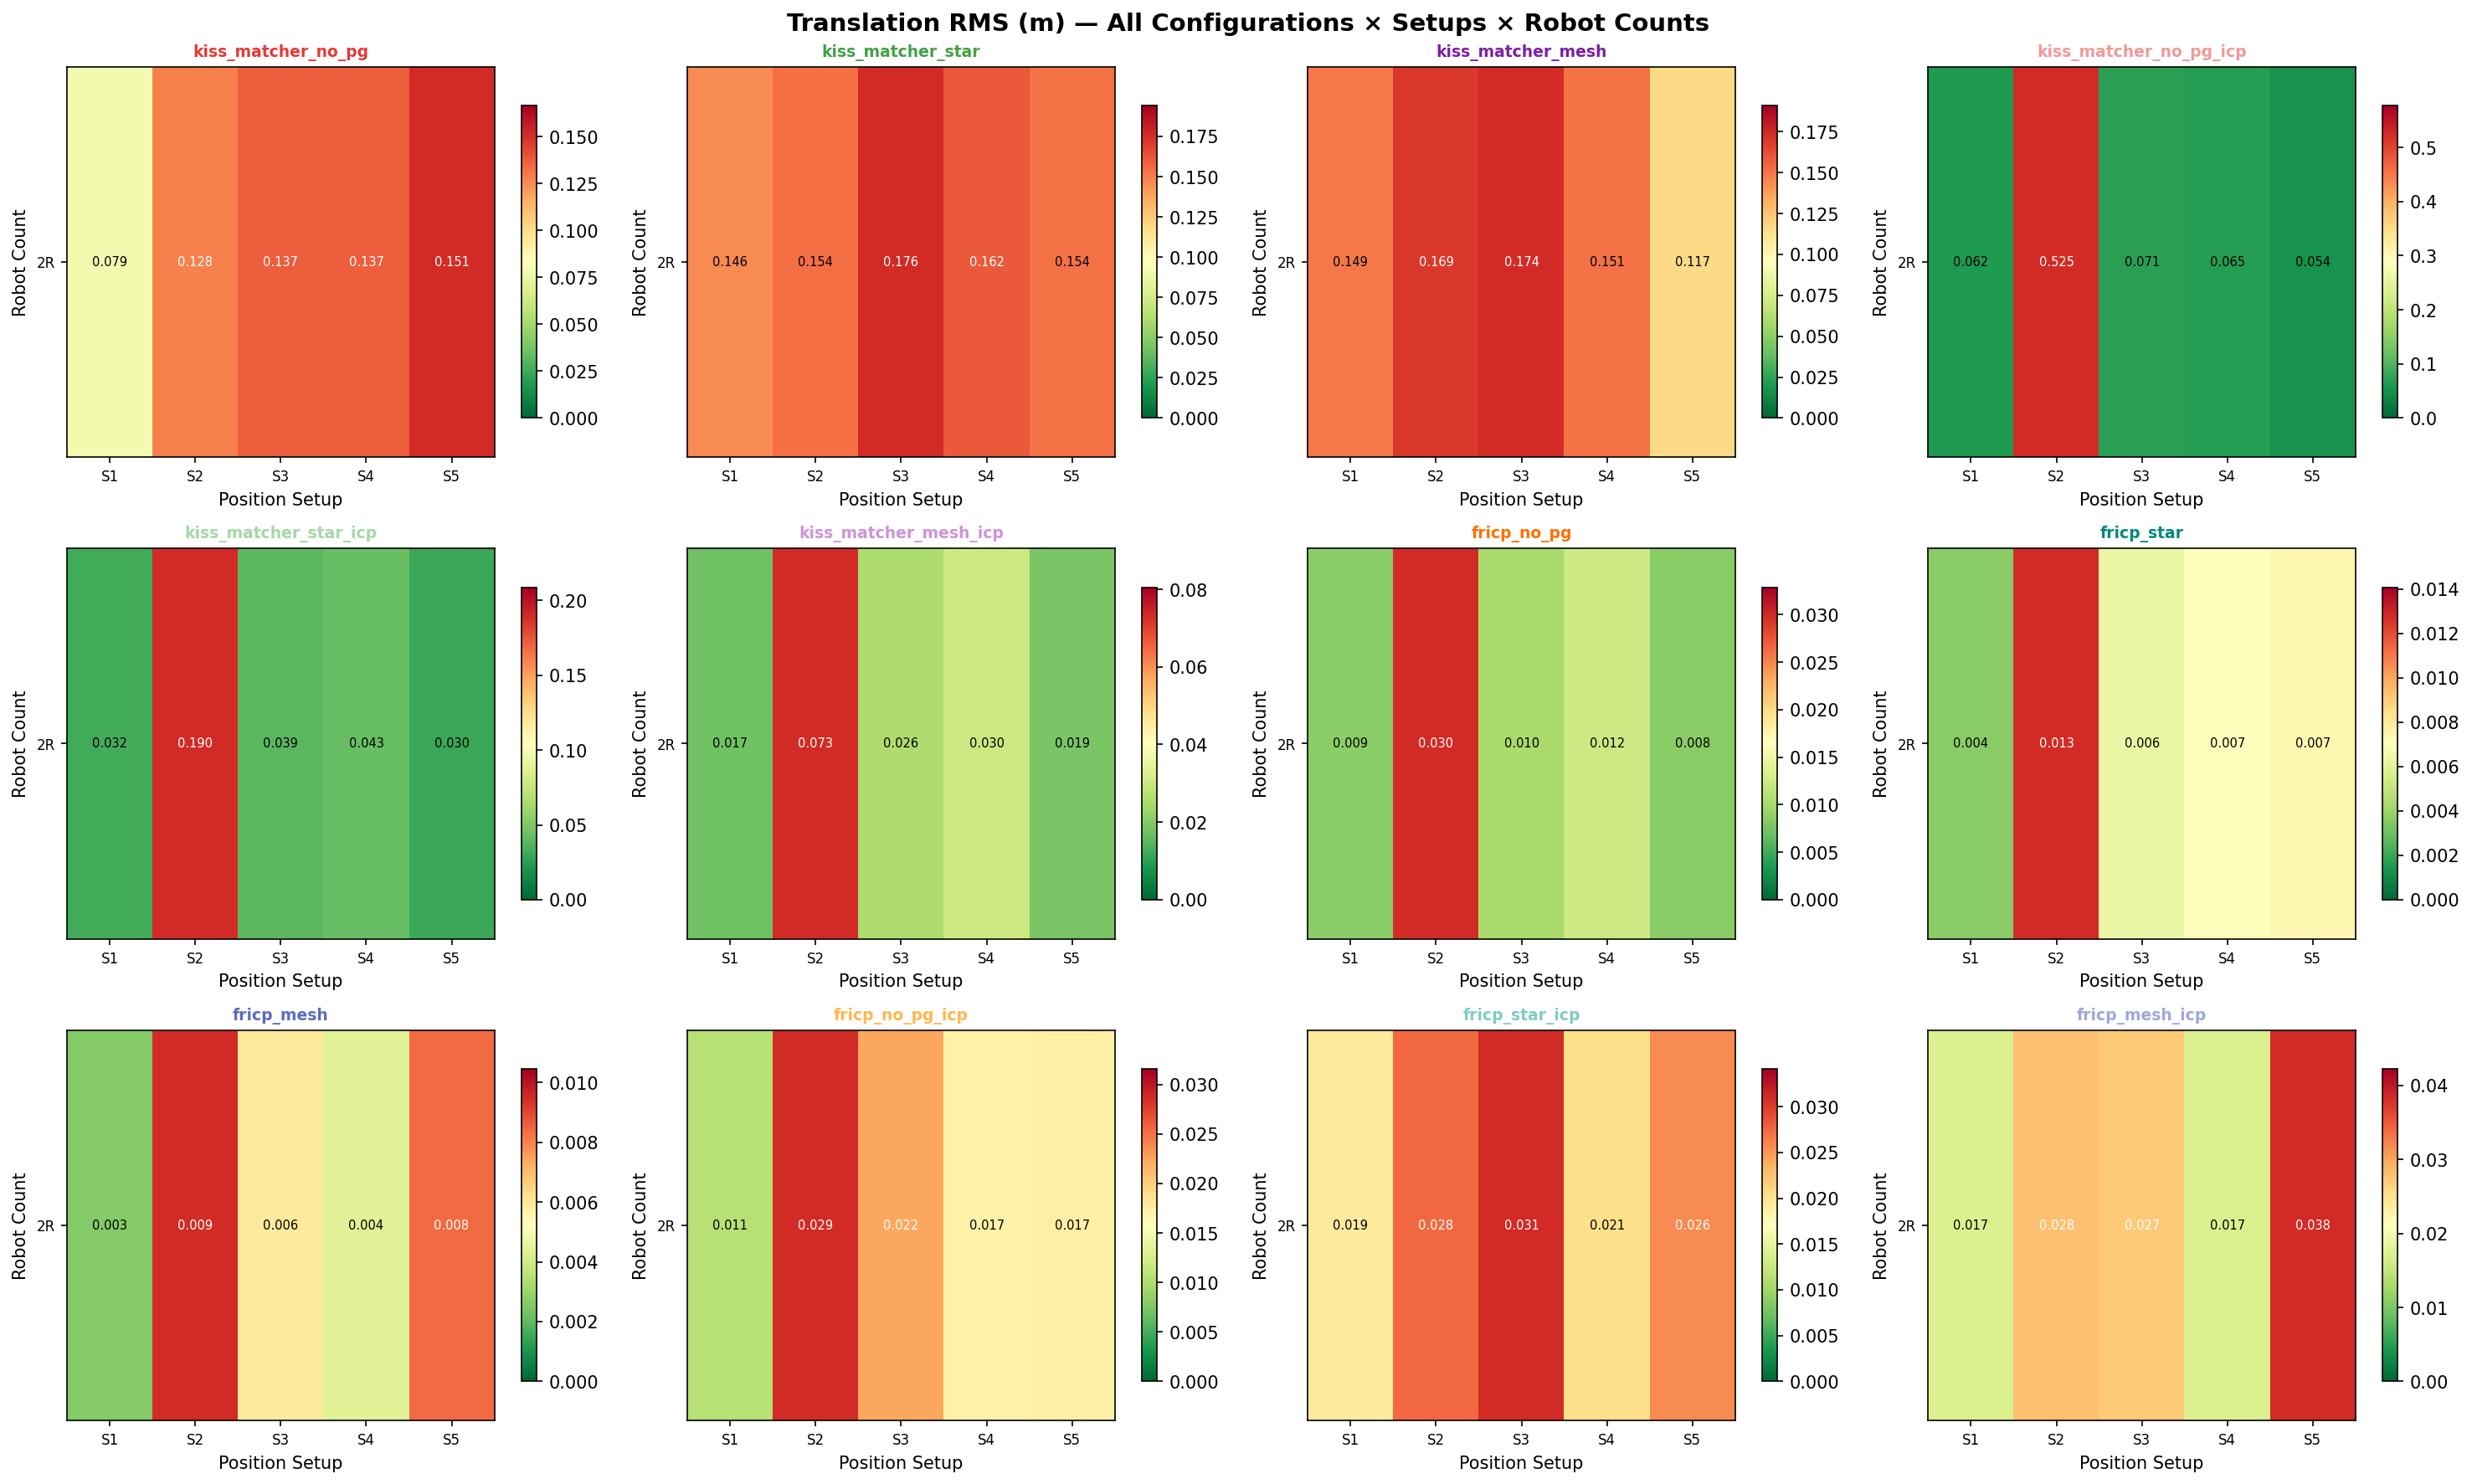
\includegraphics[width=\textwidth]{figures/heatmap_all_configs.png}
%   \caption{Heatmap of translation RMS error across robot counts and
%            position setups for all 12 configurations.
%            Green indicates low error; red indicates high error.}
%   \label{fig:heatmap}
% \end{figure}

%% ---------------------------------------------------------------------------
\section{Summary}
\label{sec:evaluation_summary}

The experimental evaluation, comprising over 900 individual
calibration runs across 2 deployment scenarios, 3 fleet sizes,
15 position setups, and 12 parameter combinations, yields the
following key findings:

\begin{enumerate}
    \item \textbf{The optimal backend depends on the deployment
          scenario.}
          In the multi-robot distributed scenario ($N \geq 3$),
          KISS-Matcher consistently outperforms FRICP, which frequently
          converges to local minima (rotation errors $> 100\degree$).
          In the two-robot proximity scenario, the result reverses:
          FRICP achieves sub-centimeter accuracy
          ($\bar{e}_t = \SI{6.2}{\milli\metre}$) while KISS-Matcher
          is limited to $\sim$\,\SI{13}{\centi\metre} by its
          feature quantization.
          The key differentiator is whether the identity transform
          provides a reasonable initial alignment (proximity) or not
          (distributed).

    \item \textbf{Pose graph optimization does not consistently improve
          accuracy in the multi-robot scenario.}
          When averaged across all position setups and fleet sizes,
          pose graph optimization degraded KISS-Matcher accuracy by
          33--55\%, as unreliable pairwise registrations in challenging
          setups propagate errors through the graph.
          For FRICP in the proximity scenario, the pose graph noise
          model provides a small improvement.
          The benefit of pose graph optimization is highly
          setup-dependent rather than universal.

    \item \textbf{ICP refinement impact is scenario-dependent.}
          In the multi-robot scenario with sparse, single-LiDAR point
          clouds, ICP degrades accuracy by up to 50\% by converging
          to locally dense regions.
          In the proximity scenario with dense $360\degree$ coverage
          and high overlap, ICP improves KISS-Matcher accuracy by
          58--78\% (with PG) but degrades FRICP, which is already
          near-optimal.

    \item \textbf{Sub-centimeter accuracy is achievable for the
          primary use case.}
          The two-robot proximity scenario---the most common real-world
          deployment---achieves $\bar{e}_t = \SI{6.2}{\milli\metre}$
          and $\bar{e}_r = 0.03\degree$ with FRICP and mesh PG,
          consistent across all five position setups
          (\SIrange{0.8}{2.0}{\metre} separation).

    \item \textbf{Results are sensitive to geometric context.}
          In the multi-robot scenario, calibration accuracy varies
          significantly across spatial arrangements (best:
          $\bar{e}_t = \SI{0.37}{\metre}$, worst:
          $\bar{e}_t = \SI{1.60}{\metre}$ for 3~robots), driven by
          the geometric features visible in each robot's LiDAR field
          of view.
          The proximity scenario is more robust, with all setups
          achieving sub-centimeter accuracy.

    \item \textbf{Recommended configurations:}
          \begin{itemize}
              \item \textbf{Two-robot proximity:} FRICP with pose graph
                    ($\bar{e}_t \approx \SI{6}{\milli\metre}$,
                    $t \approx \SI{0.8}{\second}$).
              \item \textbf{Multi-robot distributed:} KISS-Matcher
                    without pose graph
                    ($\bar{e}_t \approx \SI{2.58}{\metre}$,
                    $t \approx \SI{0.1}{\second}$).
          \end{itemize}
\end{enumerate}

%% ---------------------------------------------------------------------------
%% Bibliography entries referenced in this chapter (add to your main .bib file):
%%
%% @misc{gazebo_harmonic,
%%   title  = {Gazebo Harmonic},
%%   author = {{Open Robotics}},
%%   year   = {2024},
%%   note   = {\url{https://gazebosim.org}}
%% }
%%
%% @misc{rgl_plugin,
%%   title  = {{RGLGazeboPlugin}: Robotec {GPU} Lidar for Gazebo},
%%   author = {{Robotec.AI}},
%%   year   = {2024},
%%   note   = {\url{https://github.com/RobotecAI/RGLGazeboPlugin}}
%% }
%%
%% @misc{livox_mid360,
%%   title  = {Livox Mid-360 LiDAR},
%%   author = {{Livox Technology}},
%%   year   = {2023},
%%   note   = {\url{https://www.livoxtech.com/mid-360}}
%% }
